%%%%%%%%%%%%%%%%%%%%%%%%%%%%%%%%%%%%%%%%%
% Article Notes
% LaTeX Template
% Version 1.0 (1/10/15)
%
% This template has been downloaded from:
% http://www.LaTeXTemplates.com
%
% Authors:
% Vel (vel@latextemplates.com)
% Christopher Eliot (christopher.eliot@hofstra.edu)
% Anthony Dardis (anthony.dardis@hofstra.edu)
%
% License:
% CC BY-NC-SA 3.0 (http://creativecommons.org/licenses/by-nc-sa/3.0/)
%
%%%%%%%%%%%%%%%%%%%%%%%%%%%%%%%%%%%%%%%%%

%----------------------------------------------------------------------------------------
%	PACKAGES AND OTHER DOCUMENT CONFIGURATIONS
%----------------------------------------------------------------------------------------

\documentclass[
12pt, % Default font size is 10pt, can alternatively be 11pt or 12pt
a4paper, % Alternatively letterpaper for US letter
onecolumn, % Alternatively twocolumn
portrait % Alternatively landscape
]{article}



%%%%%%%%%%%%%%%%%%%%%%%%%%%%%%%%%%%%%%%%%
% Article Notes
% Structure Specification File
% Version 1.0 (1/10/15)
%
% This file has been downloaded from:
% http://www.LaTeXTemplates.com
%
% Authors:
% Vel (vel@latextemplates.com)
% Christopher Eliot (christopher.eliot@hofstra.edu)
% Anthony Dardis (anthony.dardis@hofstra.edu)
%
% License:
% CC BY-NC-SA 3.0 (http://creativecommons.org/licenses/by-nc-sa/3.0/)
%
%%%%%%%%%%%%%%%%%%%%%%%%%%%%%%%%%%%%%%%%%

%----------------------------------------------------------------------------------------
%	REQUIRED PACKAGES
%----------------------------------------------------------------------------------------
\usepackage{graphicx}
\usepackage{pdfpages}
\usepackage[includeheadfoot,columnsep=2cm, left=1in, right=1in, top=.5in, bottom=.5in]{geometry} % Margins

\usepackage[T1]{fontenc} % For international characters
\usepackage{XCharter} % XCharter as the main font

\usepackage{natbib} % Use natbib to manage the reference
\bibliographystyle{apalike} % Citation style

\usepackage[english]{babel} % Use english by default
\usepackage{amsmath}
%----------------------------------------------------------------------------------------
%	CUSTOM COMMANDS
%----------------------------------------------------------------------------------------

\newcommand{\articletitle}[1]{\renewcommand{\articletitle}{#1}} % Define a command for storing the article title
\newcommand{\articlecitation}[1]{\renewcommand{\articlecitation}{#1}} % Define a command for storing the article citation
\newcommand{\doctitle}{\articlecitation\ --- ``\articletitle''} % Define a command to store the article information as it will appear in the title and header

\newcommand{\datenotesstarted}[1]{\renewcommand{\datenotesstarted}{#1}} % Define a command to store the date when notes were first made
\newcommand{\docdate}[1]{\renewcommand{\docdate}{#1}} % Define a command to store the date line in the title

\newcommand{\docauthor}[1]{\renewcommand{\docauthor}{#1}} % Define a command for storing the article notes author

% Define a command for the structure of the document title
\newcommand{\printtitle}{
\begin{center}
%\textbf{\Large{\doctitle}}

\docdate

\docauthor
\end{center}
}

%----------------------------------------------------------------------------------------
%	STRUCTURE MODIFICATIONS
%----------------------------------------------------------------------------------------

\setlength{\parskip}{3pt} % Slightly increase spacing between paragraphs

% Uncomment to center section titles
%\usepackage{sectsty}
%\sectionfont{\centering}

% Uncomment for Roman numerals for section numbers
%\renewcommand\thesection{\Roman{section}}
 % Input the file specifying the document layout and structure

\usepackage{pdfpages}
\usepackage{float}
\usepackage{subfigure,amsmath,amssymb}
\usepackage{indentfirst}
%----------------------------------------------------------------------------------------
%	ARTICLE INFORMATION
%----------------------------------------------------------------------------------------

\articletitle{Intermediate Microeconomics} % The title of the article
\articlecitation{\cite{dubner1999assessing}} % The BibTeX citation key from your bibliography

\datenotesstarted{April 30, 2017} % The date when these notes were first made
\docdate{\datenotesstarted; rev. \today} % The date when the notes were lasted updated (automatically the current date)

\docauthor{Chen} % Your name

%----------------------------------------------------------------------------------------

\begin{document}
\textbf{\LARGE{\centerline{Notes on Intermediate Microeconomics\quad}}}
\\ 
\textbf{\Large{\centerline{- A Modern Approach (Hal R. Varian)}}}
\pagestyle{myheadings} % Use custom headers
\markright{\doctitle} % Place the article information into the header

%----------------------------------------------------------------------------------------
%	PRINT ARTICLE INFORMATION
%----------------------------------------------------------------------------------------

\thispagestyle{plain} % Plain formatting on the first page

\printtitle % Print the title

%----------------------------------------------------------------------------------------
%	ARTICLE NOTES
%----------------------------------------------------------------------------------------

\section*{Introduction} % Unnumbered section

The article gives a summary of several important types of goods which have typical utility functions.

%------------------------------------------------

\section{Perfect Substitudes} % Numbered section
\begin{itemize}
\item Utility function:
	\[
	u(x_1,x_2)=ax_1+bx_2.\;(x_1\ge0,x_2\ge 0)
	\]
\begin{figure}[H]
	\centering
	\subfigure[Utility function]{
		\label{Fig.sub.1}
		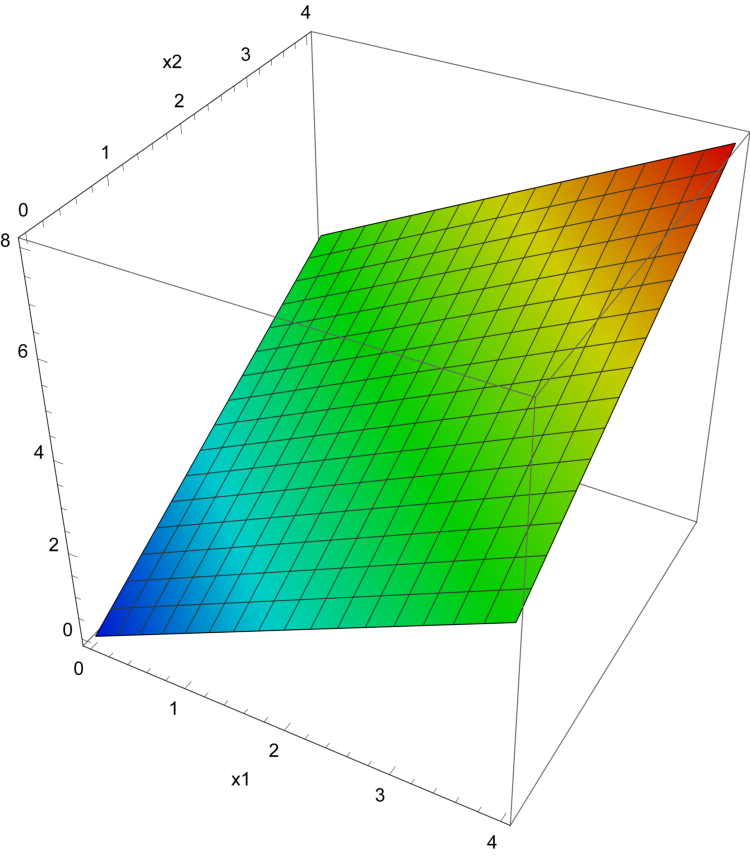
\includegraphics[width=0.55\textwidth]{PS1.pdf}}
	\subfigure[Indifference curve]{
		\label{Fig.sub.2}
		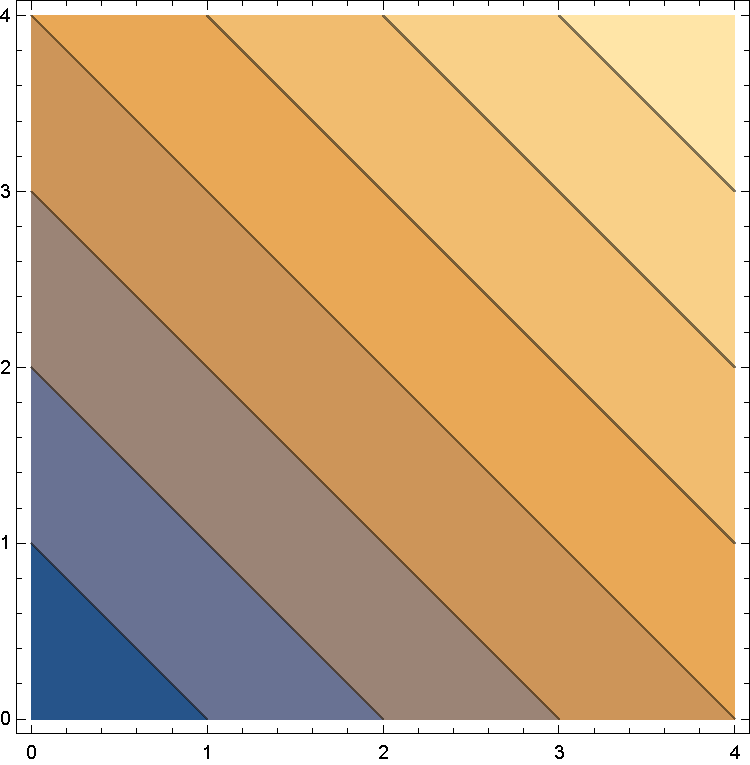
\includegraphics[width=0.35\textwidth]{PS2.pdf}}
	\caption{Utility function $u(x_1,x_2)=x_1+x_2\;(x_1\ge0,x_2\ge 0)$}
	\label{Fig.lable}
\end{figure}	


\item Maximum with budget constraint:
    
    \[
    \max_{x_1,x_2} u(x_1,x_2)=\max_{x_1,x_2}ax_1+bx_2
    \]
    \[
    \text{s.t.}\;p_1x_1+p_2x_2=w,x_1\ge0,x_2\ge 0
    \]
    \begin{enumerate}
    \item If $\dfrac{p_1}{a}<\dfrac{p_2}{b}$,
    \[
    u_{\max}=u\left(\frac{w}{p_1},0\right)=\frac{aw}{p_1}.
    \]
    \item If $\dfrac{p_1}{a}=\dfrac{p_2}{b}$, for $t\in\left[0,\dfrac{w}{p_1}\right]$
    \[
    u_{\max}=u\left(t,\frac{w-p_1t}{p_2}\right)=\frac{aw}{p_1}=\frac{bw}{p_2}.
    \]
    \item If $\dfrac{p_1}{a}>\dfrac{p_2}{b}$,
    \[
    u_{\max}=u\left(0,\frac{w}{p_2}\right)=\frac{bw}{p_2}.
    \]
    \end{enumerate}

\begin{figure}[H]
	\centering
	\subfigure[Utility function]{
		\label{Fig.sub.1}
		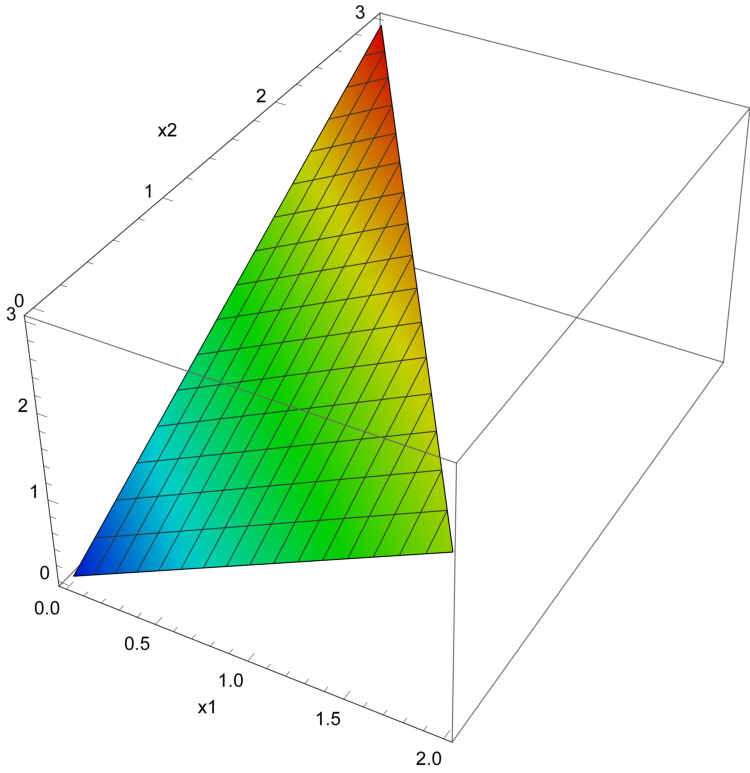
\includegraphics[width=0.6\textwidth]{PS3.pdf}}
	\subfigure[Indifference curve]{
		\label{Fig.sub.2}
		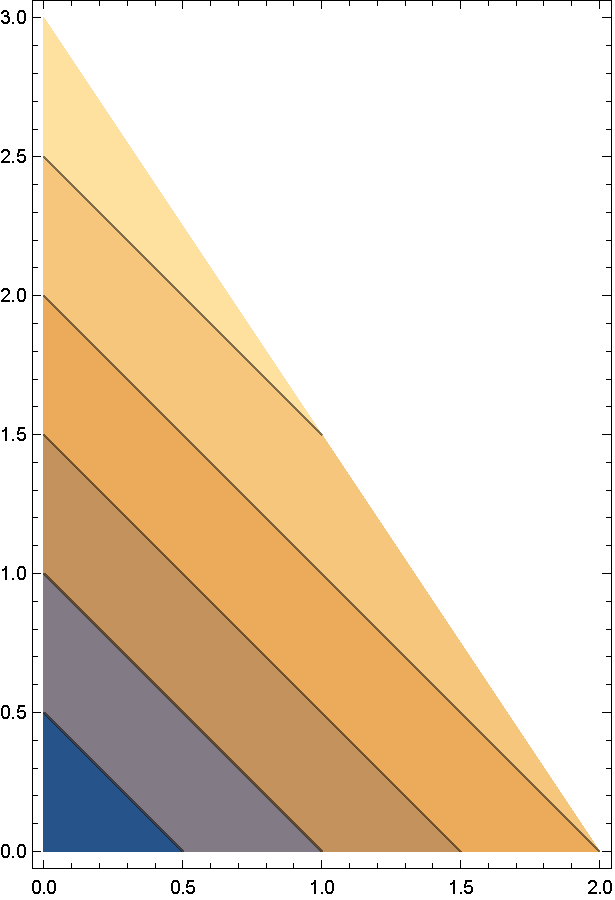
\includegraphics[width=0.3\textwidth]{PS4.pdf}}
	\caption{$u(x_1,x_2)=x_1+x_2$ s.t. $3x_1+2x_2\le 6$}
	\label{Fig.lable}
\end{figure}



\item Walras Demand function:

\begin{equation*}
x(p_1,p_2,w)=\begin{cases}
\left(\dfrac{w}{p_1},0\right)&\text{if}\;\,\dfrac{p_1}{a}<\dfrac{p_2}{b},\\
\{(x_1,x_2)\in\mathbb{R}^2_+|p_1x_1+p_2x_2=w\}&\text{if}\;\, \dfrac{p_1}{a}=\dfrac{p_2}{b},\\
\left(0,\dfrac{w}{p_2}\right)&\text{if}\;\,\dfrac{p_1}{a}>\dfrac{p_2}{b}.
\end{cases}
\end{equation*}
   

\item Indirect Utility Function:

\begin{equation*}
v(p_1,p_2,w)=\left\{
\begin{aligned}
\dfrac{aw}{p_1}\qquad&\text{if}\;\,\dfrac{p_1}{a}<=\dfrac{p_2}{b},\\
\dfrac{bw}{p_2}\qquad&\text{if}\;\,\dfrac{p_1}{a}>\dfrac{p_2}{b}.
\end{aligned}
\right.
\end{equation*}

\item Hicks Demand Function

\begin{equation*}
h(p_1,p_2,u)=\begin{cases}
\left(\dfrac{w}{p_1},0\right)&\text{if}\;\,\dfrac{p_1}{a}<\dfrac{p_2}{b},\\
\{(x_1,x_2)\in\mathbb{R}^2_+|p_1x_1+p_2x_2=w\}&\text{if}\;\, \dfrac{p_1}{a}=\dfrac{p_2}{b},\\
\left(0,\dfrac{w}{p_2}\right)&\text{if}\;\,\dfrac{p_1}{a}>\dfrac{p_2}{b}.
\end{cases}
\end{equation*}

\item Expenditure Function 

\begin{equation*}
e(p_1,p_2,u)=\begin{cases}
\left(\dfrac{w}{p_1},0\right)&\text{if}\;\,\dfrac{p_1}{a}<\dfrac{p_2}{b},\\
\{(x_1,x_2)\in\mathbb{R}^2_+|p_1x_1+p_2x_2=w\}&\text{if}\;\, \dfrac{p_1}{a}=\dfrac{p_2}{b},\\
\left(0,\dfrac{w}{p_2}\right)&\text{if}\;\,\dfrac{p_1}{a}>\dfrac{p_2}{b}.
\end{cases}
\end{equation*}

\end{itemize}




\section{Perfect Complements}


\begin{itemize}
	\item Utility function:
	\[
	u(x_1,x_2)=\min\{ax_1,bx_2\}.\;(x_1\ge0,x_2\ge 0)
	\]
	\begin{figure}[H]
		\centering
		\subfigure[Utility function]{
			\label{Fig.sub.1}
			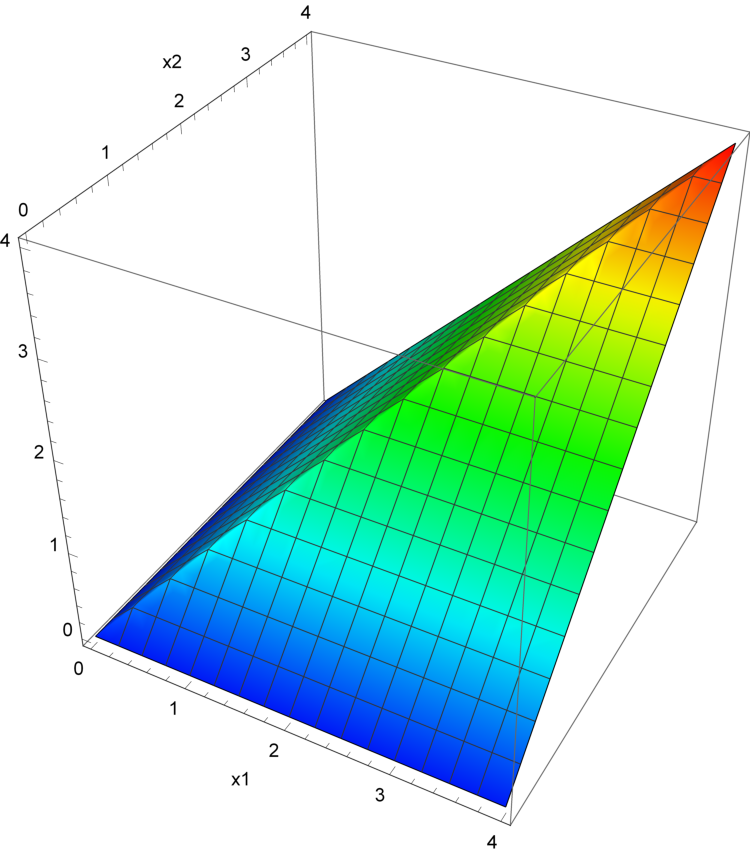
\includegraphics[width=0.55\textwidth]{PC1.pdf}}
		\subfigure[Indifference curve]{
			\label{Fig.sub.2}
			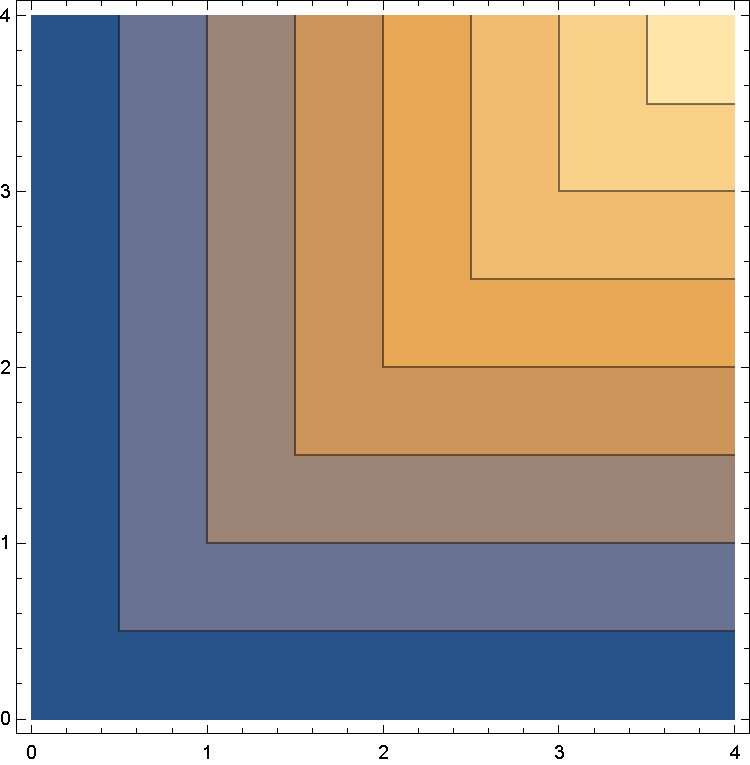
\includegraphics[width=0.35\textwidth]{PC2.pdf}}
		\caption{Utility function $u(x_1,x_2)=\min\{x_1,x_2\}$}
		\label{Fig.lable}
	\end{figure}	
	
	
	\item Maximum with budget constraint:
	
	\[
	\max_{x_1,x_2} u(x_1,x_2)=\max_{x_1,x_2}\min\{ax_1,bx_2\}
	\]
	\[
	\text{s.t.}\;p_1x_1+p_2x_2=w,x_1\ge0,x_2\ge 0.
	\]

	\[
	u_{\max}=u\left(\frac{bw}{bp_1+ap_2}\;,\;\frac{aw}{bp_1+ap_2}\right)=\frac{abw}{bp_1+ap_2}
	\]
	\begin{figure}[H]
		\centering
		\subfigure[Utility function]{
			\label{Fig.sub.1}
			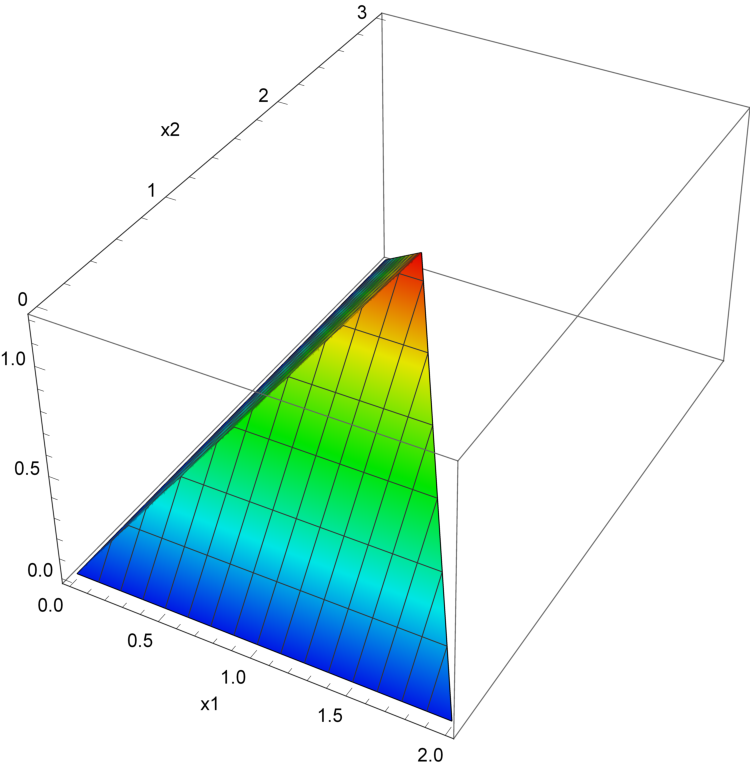
\includegraphics[width=0.6\textwidth]{PC3.pdf}}
		\subfigure[Indifference curve]{
			\label{Fig.sub.2}
			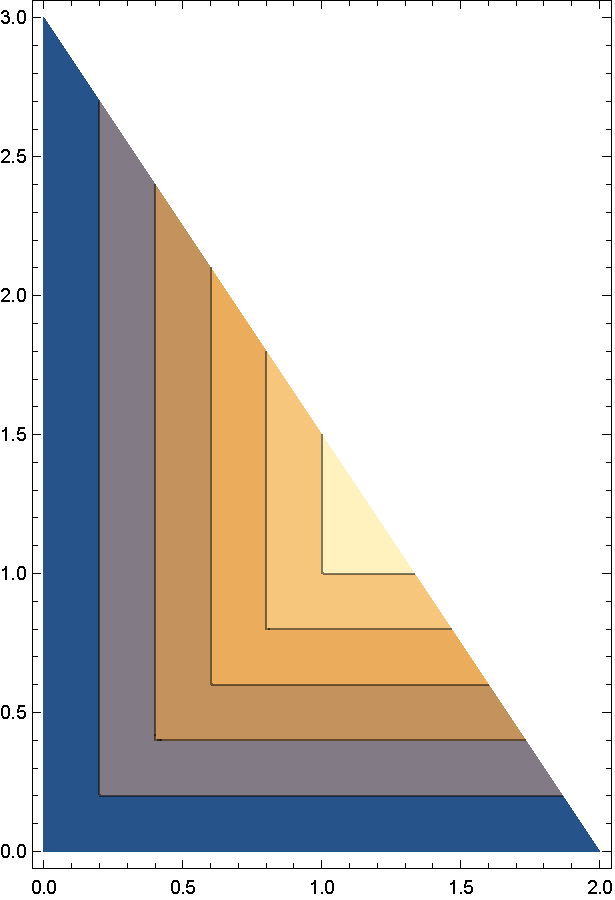
\includegraphics[width=0.3\textwidth]{PC4.pdf}}
		\caption{$u(x_1,x_2)=\min\{x_1,x_2\}$ s.t. $3x_1+2x_2\le 6$}
		\label{Fig.lable}
	\end{figure}
	
	
	


\item Walras Demand function:

\begin{equation*}
x(p_1,p_2,w)=
\left(\frac{bw}{bp_1+ap_2},\frac{aw}{bp_1+ap_2}\right)
\end{equation*}


\item Indirect Utility Function:

\begin{equation*}
v(p_1,p_2,w)=\frac{2abw}{bp_1+ap_2}
\end{equation*}
	
\end{itemize}





\section{Cobb-Douglas Preference}

\begin{itemize}
	\item Utility function:
	\[
	u(x_1,x_2)=x_1^cx_2^d.\;(x_1\ge0,x_2\ge 0)
	\]
	
	\begin{figure}[H]
		\centering
		\subfigure[Utility function]{
			\label{Fig.sub.1}
			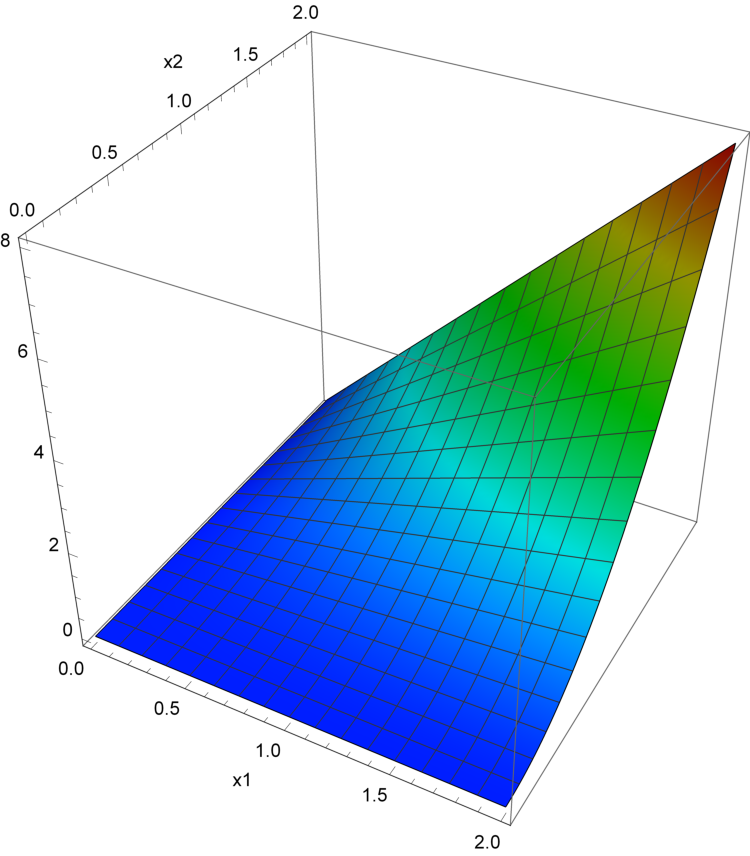
\includegraphics[width=0.55\textwidth]{CD1.pdf}}
		\subfigure[Indifference curve]{
			\label{Fig.sub.2}
			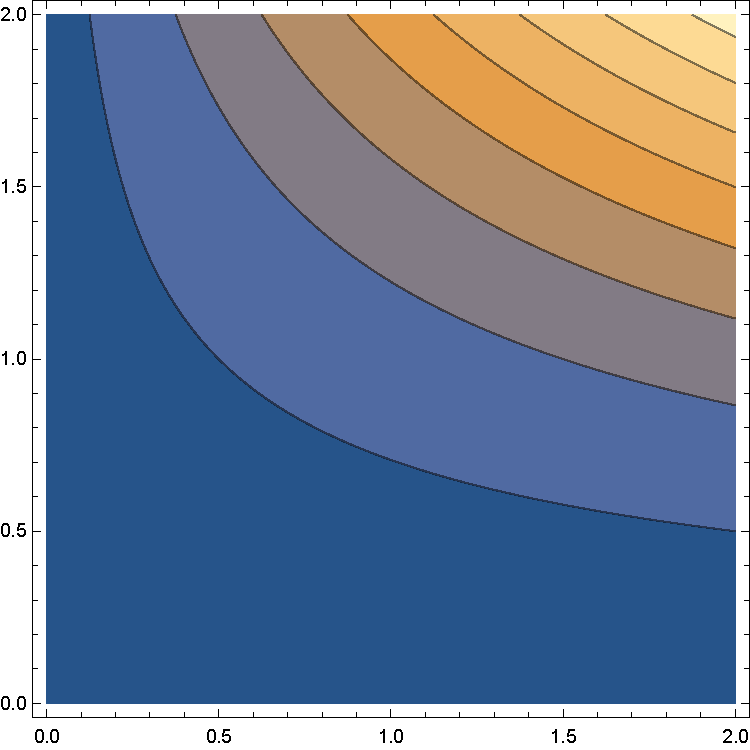
\includegraphics[width=0.35\textwidth]{CD2.pdf}}
		\caption{Utility function $u(x_1,x_2)=x_1x_2^{2}$}
		\label{Fig.lable}
	\end{figure}
	
	\item Maximum with budget constraint:
	\[
	\max_{x_1,x_2} u(x_1,x_2)=\max_{x_1,x_2}x_1^cx_2^d
	\]
	\[
	\text{s.t.}\;p_1x_1+p_2x_2=w.
	\]
	
	\[
	u_{\max}=u\left(\frac{c}{c+d}\cdot\frac{w}{p_1}\;,\;\frac{d}{c+d}\cdot\frac{w}{p_2}\right)=\left(\frac{w}{c+d}\right)^{c+d}\frac{c^cd^d}{p_1^c\,p_2^d}.
	\]
	
	\begin{figure}[H]
		\centering
		\subfigure[Utility function]{
			\label{Fig.sub.1}
			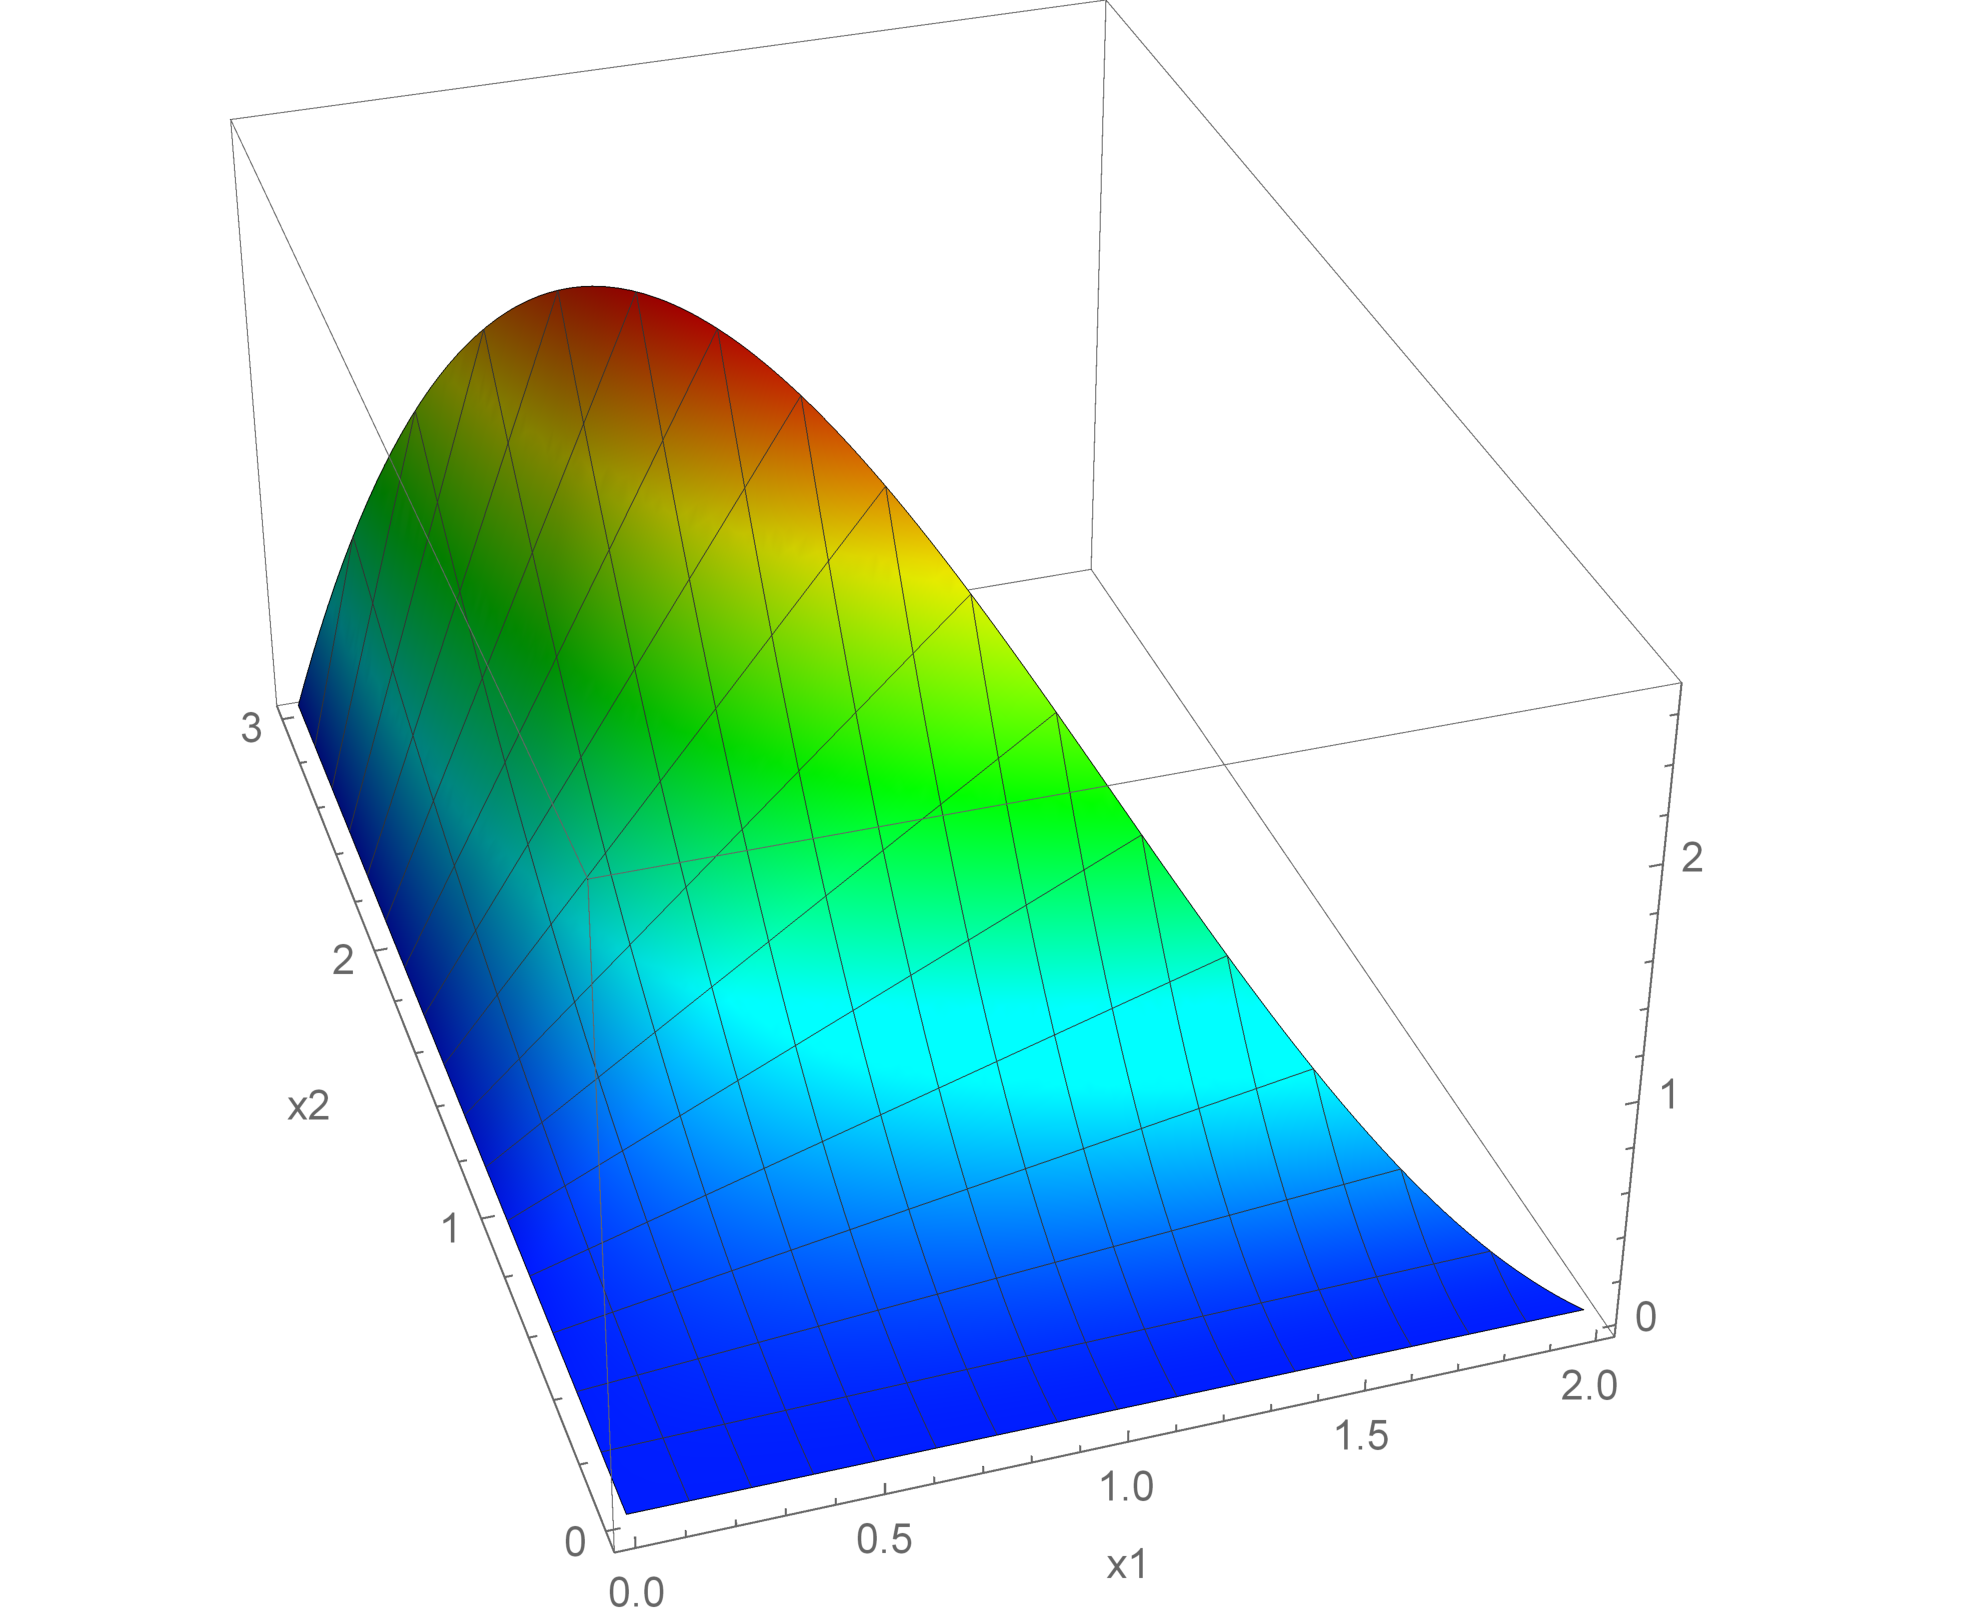
\includegraphics[width=0.6\textwidth]{CD3.pdf}}
		\subfigure[Indifference curve]{
			\label{Fig.sub.2}
			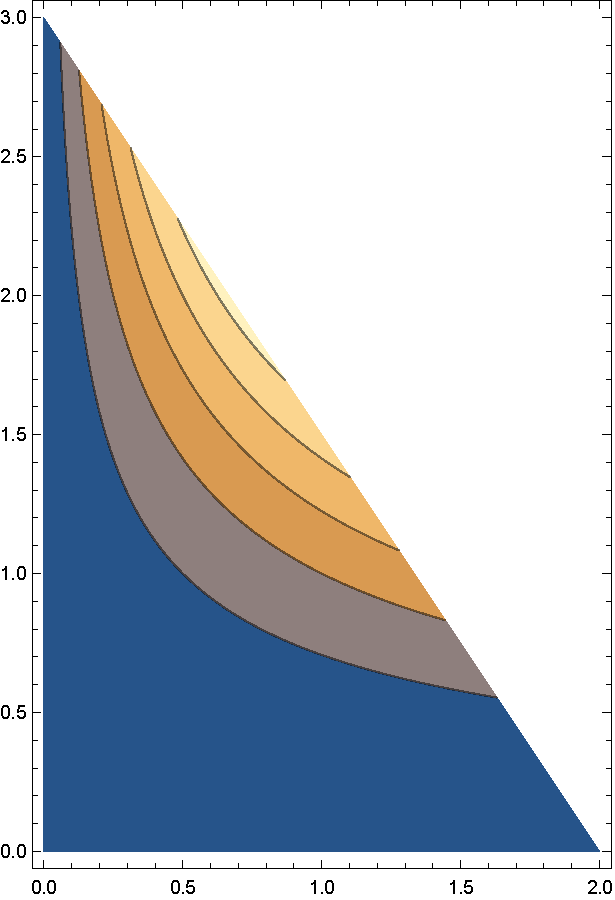
\includegraphics[width=0.3\textwidth]{CD4.pdf}}
		\caption{$u(x_1,x_2)=x_1x_2^2$ s.t. $3x_1+2x_2\le 6$}
		\label{Fig.lable}
	\end{figure}
	
	\item Walras Demand function
	\[
	x(p_1,p_2,w)=\left(\frac{c}{c+d}\cdot\frac{w}{p_1},\frac{d}{c+d}\cdot\frac{w}{p_2}\right),
	\]
	\item Indirect Utility Function:
	\[
	v(p_1,p_2,w)=\frac{ac}{c+d}\cdot\frac{w}{p_1}+\frac{bd}{c+d}\cdot\frac{w}{p_2}
	\]

\end{itemize}


\section{Quasilinear Preference}
\begin{itemize}
	
\item Utility function:
\[
u(x_1,x_2)=x_1+\ln x_2.\;(x_1\ge0,x_2> 0)
\]

\begin{figure}[H]
	\centering
	\subfigure[Utility function]{
		\label{Fig.sub.1}
		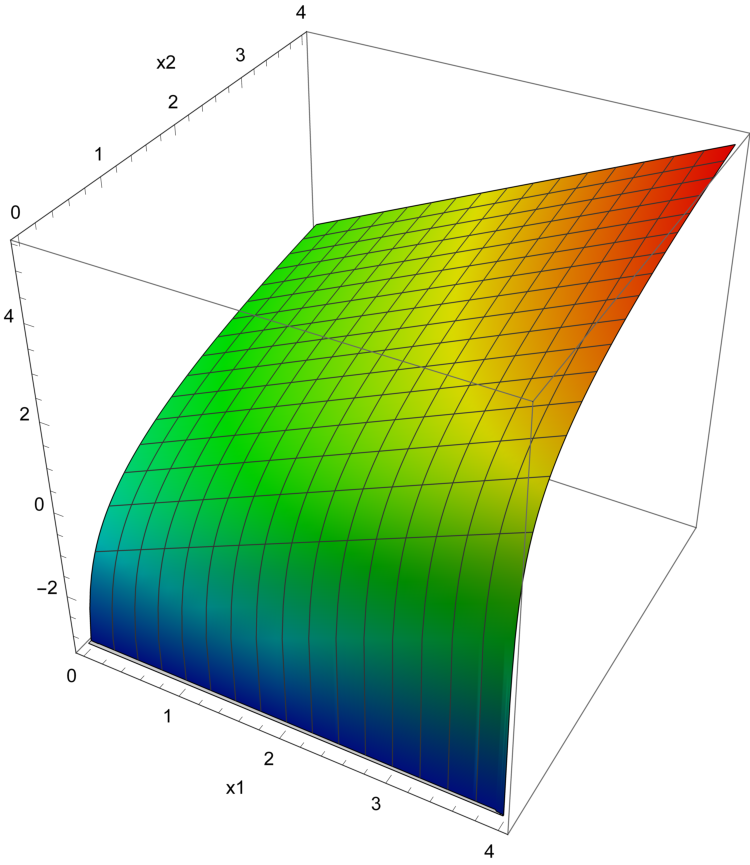
\includegraphics[width=0.55\textwidth]{QL1.pdf}}
	\subfigure[Indifference curve]{
		\label{Fig.sub.2}
		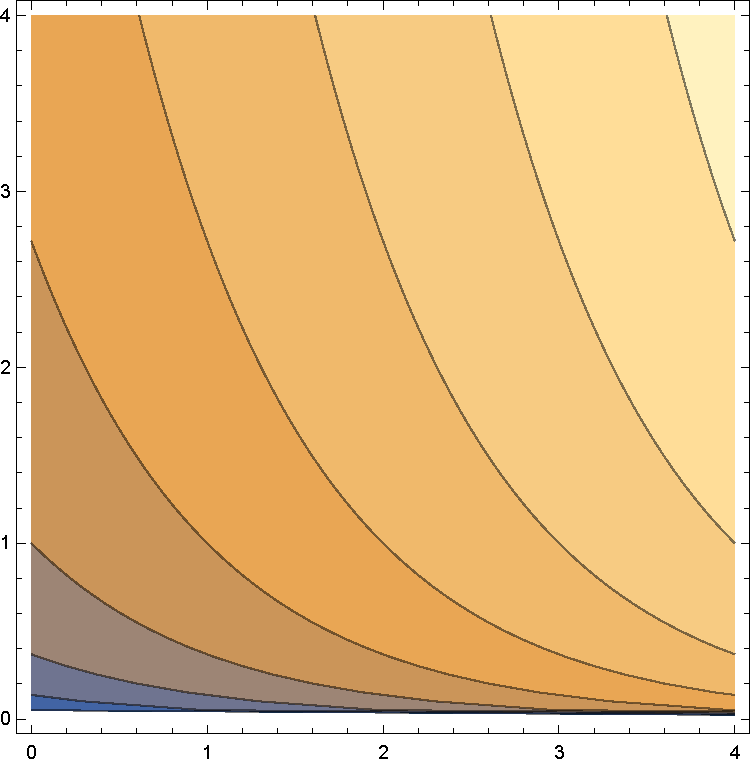
\includegraphics[width=0.35\textwidth]{QL2.pdf}}
	\caption{Utility function $u(x_1,x_2)=x_1+\ln x_2$}
	\label{Fig.lable}
\end{figure}

\item Maximum with budget constraint:
\[
\max_{x_1,x_2} u(x_1,x_2)=x_1+\ln x_2
\]
\[
\text{s.t.}\;p_1x_1+p_2x_2\le w.
\]

\begin{figure}[H]
	\centering
	\subfigure[Utility function]{
		\label{Fig.sub.1}
		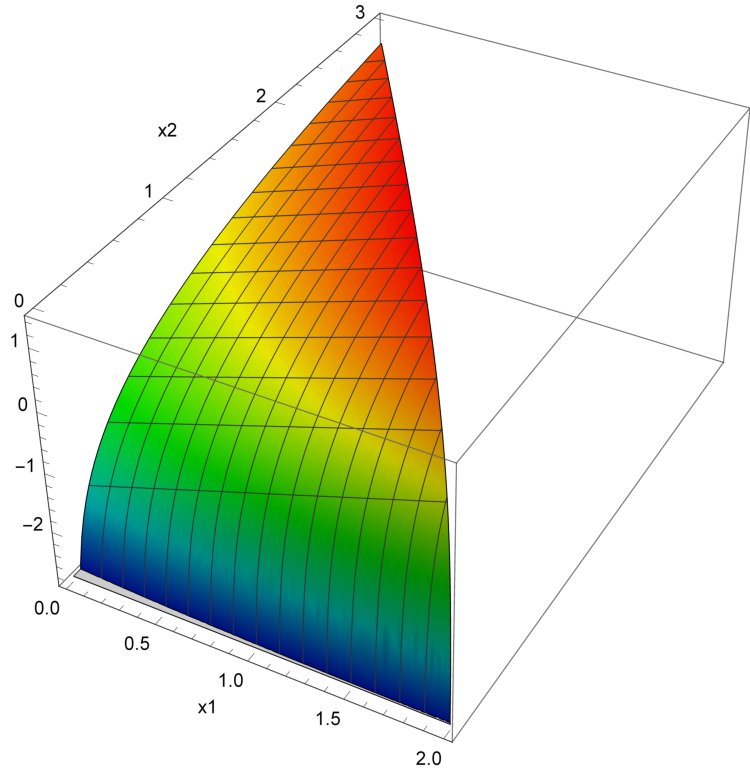
\includegraphics[width=0.55\textwidth]{QL3.pdf}}
	\subfigure[Indifference curve]{
		\label{Fig.sub.2}
		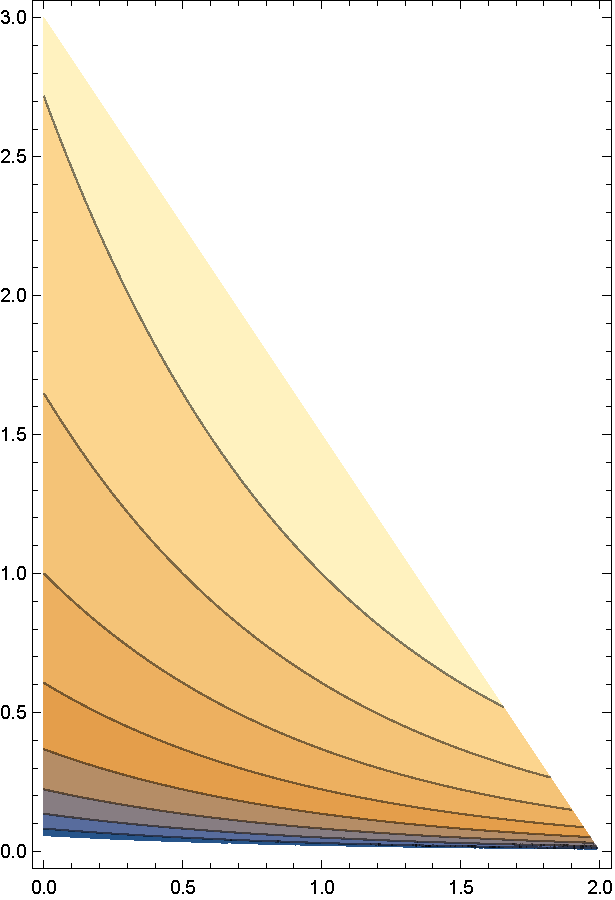
\includegraphics[width=0.35\textwidth]{QL4.pdf}}
	\caption{Utility function $u(x_1,x_2)=x_1+\ln x_2$}
	\label{Fig.lable}
\end{figure}
	
\item Walras Demand function
\begin{equation*}
x(p_1,p_2,w)=\left\{
\begin{aligned}
&\left(0,\dfrac{w}{p_2}\right)&\text{if}\;\,w<p_1,\\
&\left(\dfrac{w-p_1}{p_1},\dfrac{p_1}{p_2}\right)&\text{if}\;\,w\ge p_1.
\end{aligned}
\right.
\end{equation*}

\item Indirect Utility Function:
\begin{equation*}
v(p_1,p_2,w)=\left\{
\begin{aligned}
&\ln\dfrac{w}{p_2}&\text{if}\;\,w<p_1,\\
&\dfrac{w-p_1}{p_1}+\ln\dfrac{p_1}{p_2}&\text{if}\;\,w\ge p_1.
\end{aligned}
\right.
\end{equation*}

\end{itemize}










%----------------------------------------------------------------------------------------
%	BIBLIOGRAPHY
%----------------------------------------------------------------------------------------

%\renewcommand{\refname}{Reference} % Change the default bibliography title

%\bibliography{sample} % Input your bibliography file

%----------------------------------------------------------------------------------------

\end{document}